
\section{Geometría euclídea}

Llamamos geometría euclídea al espacio en el que podemos medir, cosa que hasta ahora no era posible.

Todo surge desde el módulo de un vector. Llamamos \concept[Módulo de un vector]{módulo de un vector} a la longitud que tiene. Dado $\vec{v}$, se define el módulo como $|\vec{v}|$.

Si el vector $\vec{v}$ tiene como coordenadas $\vec{v} = (v_1,v_2,v_3)$ en la base canónica, podemos calcular su módulo como $|\vec{v}| = \sqrt{v_1^2+v_2^2+v_3^2}$

\begin{prop}
$\left|\lambda\vec{v}\right| = |\lambda|·|\vec{v}|$
\end{prop}
\begin{proof}
$$|\lambda·\vec{v}| = \sqrt{(\lambda·v_1)^2+(\lambda·v_2)^2+(\lambda·v_3)^2} = \sqrt{\lambda^2 (v_1^2+v_2^2+v_3^2)} = |\lambda| ·\left|\vec{u}\right|$$
\end{proof}

\begin{defn}[Vector\IS unitario]
\[\vec{u}\in V^3 \text{ es unitario } \dimplies \left|\vec{u}\right|=1\]
\end{defn}

\begin{problem}
Dado el vector $\vec{u} = (0,3,4)$, encuentra:
\ppart Un vector unitario con la misma dirección. ¿Cuántos hay?
\ppart Un vector unitario con la misma dirección y el mismo sentido. ¿Cuántos hay?
\solution

Calculamos $\vec{u} = \sqrt{0^2+3^2+4^5} = \sqrt{25} = 5$

\spart Buscamos $\vec{v} = (0,3\lambda,4\lambda)$ tal que $|\vec{v}| = 1$

\[|\vec{v}| = \sqrt{0^2+(3\lambda)^2+(4\lambda)^2} = \sqrt{25\lambda^2} =1 \dimplies \lambda=\pm\rfrac{1}{5}\]

Hay dos vectores unitarios ocn la misma dirección: $\vec{v_1} = \left(0,\rfrac{3}{5},\rfrac{4}{5}\right)$ y $\vec{v_2} = \left(0,-\rfrac{3}{5},-\rfrac{4}{5}\right)$

Hay 2 vectores unitarios con la misma dirección.

\obs Estos dos vectores tienen la misma dirección pero sentido contrario.

\spart El único vector unitario con la misma dirección y el mismo sentido es $\vec{v_2}$

\end{problem}

\obs ¿Es casualidad que $\lambda = \rfrac{1}{\left|\vec{u}\right|}$?  

\begin{prop}
Dado $\vec{u} = (u_1,u_2,u_3)$
\[\text{El vector } \frac{1}{\left|\vec{u}\right|}\vec{u} = \left(\frac{u_1}{\left|\vec{u}\right|},\frac{u_2}{\left|\vec{u}\right|},\frac{u_3}{\left|\vec{u}\right|}\right)\text{ es unitario}\]
\end{prop}

\begin{proof}
Para demostrarlo solamente es necesario aplicar la propiedad del módulo: $\left|\lambda·\vec{u}\right| = |\lambda|·\left|\vec{u}\right|$

\[\left|\frac{1}{\left|\vec{u}\right|}\vec{u}\right| = \frac{1}{\left|\vec{u}\right|}\left|\vec{u}\right| = 1\]
\end{proof}

\subsection{Productos (escalar, vectorial y mixto)}

% \paragraph{Introducción sobre el origen del producto escalar y vectorial}

% Fuentes consultadas:
% \begin{itemize}
%   \item \href{http://www.suitcaseofdreams.net/Geometric_multiplication.htm}{Relación forma polar y binómica del producto complejo}
%   \vspace{-0.4cm}
%   \item \href{https://www2.clarku.edu/faculty/djoyce/complex/mult.html}{Interpretación geométrica del producto complejo}
%   \vspace{-0.4cm}
%   \item \href{https://www.quora.com/Who-invented-the-dot-product-and-cross-product}{Historia y aplicación de los cuaterniones los productos}
%   \vspace{-0.4cm}
%   \item \href{https://es.wikipedia.org/wiki/Cuaterni%C3%B3n}{ Extensión de los complejos al grupo de los quaterniones}
% \end{itemize}

% Dados 2 números complejos $z_1 = a_1+b_1i$, $z_2 = a_2+b_2i$. Expresando estos números complejos en forma polar tenemos: $z_1=r_{\alpha_1}$ y $z_2 = s_{\alpha_2}$.  

% $z_1·z_2 = (a_1a_2 - b_1b_2) + (a_1b_2+a_2b_1)i = r·s_{\alpha_1+\alpha_2}$.

% Tomando $z_1·\bar{z_2} = (a_1a_2 + b_1b_2) + (a_1b_2-a_2b_1)i = r·s_{\alpha_1-\alpha_2}
% $

% \subparagraph{Estudio de la parte real (producto escalar)}

% En $Re(z_1·\bar{z_2}) = a_1a_2 + b_1b_2 = Re(r·s_{\alpha_1-\alpha_2})$

% Para calcular $Re(r·s_{\alpha_1-\alpha_2}) = Re(r·s·\cos(\alpha_1-\alpha_2) + i·r·s·\sen(\alpha_1-\alpha_2)$, por lo que podemos completar:

% $ a_1a_2 + b_1b_2 = |z_1\;||\;z_2|·\cos(\alpha_1-\alpha_2)$, y, siendo conscientes que $\alpha_1-\alpha_2$ es el ángulo que forman los 2 vectores, obtenemos la expresión del producto escalar de 2 vectores.


% \subparagraph{Estudio de la parte imaginaria (producto vectorial)}

% Al extender este razonamiento al grupo de los cuaterniones, tendríamos:

% \newcommand{\quat}{\vec}

% $Re(z_1\bar{z_2}) = Re\left((b_1\quat{i}+c_1\quat{j}+d_1\quat{k})·(-b_2\quat{i}-c_2\quat{j}-d_2\quat{k})\right) = (b_1b_2+c_1c_2+d_1d_2)$

% Lo espectacular viene al considerar la parte "imaginaria" (aunque no tengamos claro cómo se define ese concepto en los cuaterniones):

% $Im(z_1\bar{z_2}) = f(\quat{i},\quat{j},\quat{k})$, cuya expresión analítica es la del producto vectorial, ya que en grupo de los cuaterniones $\quat{i}\quat{j}=\quat{k}$ y todo eso.

\subsubsection{Producto escalar}

\begin{defn}[Producto\IS escalar]

Dados $\vec{v},\vec{w}$, se define $\appl{\cdot}{V^3\times V^3}{\real}$ como 
\[\vec{v}·\vec{w} = |\vec{w}|·|\vec{v}|\cdot\cos\left(\widehat{\vec{v},\vec{w}}\right)\]
\end{defn}

\paragraph{Propiedades:} $\forall\vx,\vx,\vz\in V^3$

\begin{itemize}
  \item \textbf{Conmutativo: } $\vx·\vy = \vy·\vx$
  \item \textbf{Bilineal:}
  \subitem  $(λ\vx)·\vy=λ(\vx·\vy)$
  \subitem  $\vx·(\vy+\vz) = \vx·\vy + \vx·\vz$
  \item \textbf{No negatividad:} $\vx·\vx ≥0$
\end{itemize}


¿Qué ocurre si no cooncemos el ángulo que forman los 2 vectores? Necesitamos otra manera de calcular el producto escalar. 

\begin{prop}[Expresión analítica del producto\IS escalar]

Dados $\vec{v}=(v_1,v_2,v_3),\vec{w}=(w_1,w_2,w_3)\in V^2$ respecto de la base canónica $\mathcal{B} = \{\vi,\vj,\vk\}$, entonces $\vec{v}·\vec{w} = v_1·w_1 + v_2·w_2+ v_3·w_3$
\end{prop}

\begin{proof}

\[
\vec{v}·\vec{w} = \left(v_1\vi+v_2\vj+v_3\vk\right)·\left(w_1\vi+w_2\vj+w_3\vk\right)\]
\[
v_1w_1\vi\vi+v_1w_2\vi\vj+v_1w_3\vi\vz+\]\[
v_2w_1\vj\vi+v_2w_2\vj\vj+v_2w_3\vj\vz+\]\[
v_3w_1\vz\vi+v_3w_2\vz\vj+v_3w_3\vz\vz = 
\]
\[
v_1w_1+v_1w_2·0+v_1w_3·0+\]\[
v_2w_1·0+v_2w_2+v_2w_3·0+\]\[
v_3w_1·0+v_3w_2·0+v_3w_3= \]
\[v_1·w_1 + v_2·w_2 + w_3·v_3\]
\end{proof}


\begin{prop} 
\[
\vec{u}·\vec{u} = \left|\vec{u}\right|^2
\]
\end{prop}


\begin{defn}[Ortogonalidad y perpendicularidad]

Decimos que $\vec{u},\vec{v}\in V^3$ son \textbf{perpendiculares} si forman un ángulo recto. Escribiremos $\vec{u}\perp\vec{v}$.

Decimos que $\vec{u},\vec{v}\in V^3$ son \textbf{ortogonales} si $\vec{u}·\vec{v} = 0$
\end{defn}

\obs Hay ligero matiz. Fíjate que $\vec{u}\perp\vec{v} \implies \vec{u}·\vec{v} = 0$ pero no al revés, ya que $\vec{0} = (0,0)$ es ortogonal a todos pero perpendicular a ninguno.

\paragraph{Clasificación de bases de vectores}

Dada la base $\mathcal{B} = \left\{\vec{a},\vec{b},\vec{c}\right\}$.

\begin{itemize}
  \item Decimos que es una base \concept[Base\IS ortogonal]{ortogonal} si y solo si $\vec{a}\perp\vec{b}\perp\vec{c}$.
  \item Decimos que es una base \concept[Base\IS ortonormal]{ortonormal} si y solo si es una base ortogonal y $|\vec{a}| = |\vec{b}| = |\vec{c}|$
\end{itemize}


\obs Con el producto escalar podemos calcular el \concept[Angulo entre\IS vectores]{angulo que forman 2 vectores}. Dado que $\vec{u}·\vec{v} = \left|\vec{u}\right|·\left|\vec{u}\right|·\cos\left(\widehat{\vec{u},\vec{v}}\right)$, podemos despejar 

\[\cos\left(\widehat{\vec{u},\vec{v}}\right) = \frac{\vec{u}·\vec{v}}{\left|\vec{u}\right|·\left|\vec{u}\right|}\]


\begin{problem}

Halla el ángulo que forman los vectores $\vec{u}=\left(2,-3,1\right),\vec{v}=\left(1,2,-2\right)$


\solution


\[\cos\left(\widehat{\vec{u},\vec{v}}\right) = \frac{\vec{u}·\vec{v}}{\left|\vec{u}\right|·\left|\vec{u}\right|} = \frac{2·1-3·2+1·(-2)}{\sqrt{14}{\sqrt{9}}} = \frac{-2}{\sqrt{14}}\]

Para calcular el ángulo que forman: 

\[
\widehat{\vec{u},\vec{v}} = \arccos \frac{-2}{\sqrt{14}} = 122º 19'
\]
\end{problem}

\begin{problem}

Halla el valor de $k$ para que el ángulo que forman los vectores $\vec{a} = (1,k,k)$ y $\vec{b} = (1,-2,1)$ sea de 60º. 
\solution
$k=-\rfrac{1}{2}$

\end{problem}

\paragraph{Interpretación geométrica del producto escalar}

\hl{Por terminar}

\subsubsection{Producto vectorial}


\begin{defn}[Producto\IS vectorial]
Dados $\vec{v},\vec{w}$, se define $\appl{\times}{V^3\times V^3}{V^3}$ como 
\[\vec{v}\times\vec{w} = |\vec{w}|·|\vec{v}|\cdot\sen\left(\widehat{\vec{v},\vec{w}}\right)·\vec{n}\]

donde $\vec{n}$ es un vector unitario y ortogonal a $\vec{v},\vec{w}$ y su sentido está dado por la regla de la \textit{mano derecha}.
\end{defn}

\paragraph{Propiedades:} $\forall\vx,\vx,\vz\in V^3$

\begin{itemize}
  \item \textbf{Anticonmutativo: } $\vx\times\vy = -\vy\times\vx$ 
  \subitem Al alterar el orden del producto, el sentido del vector resultante es contrario.
  \item \textbf{Homogénea:} $(λ\vx)\times\vy=λ(\vx\times\vy)$
  \item\textbf{Distributiva:}  $\vx\times(\vy+\vz) = \vx\times\vy + \vx\times\vz$
  \item $\vx\times\vx=0$
  \subitem Dados dos vectores $\vv\neq0$ y $\vw \vv\times\vw = 0 \dimplies \vv\;||\;\vw$
\end{itemize}

\begin{prop}[Expresión analítica del producto\IS vectorial]

Dados $\vec{v}=(v_1,v_2,v_3),\vec{w}=(w_1,w_2,w_3)\in V^2$ respecto de la base canónica $\mathcal{B} = \{\vi,\vj,\vk\}$, entonces 
\[\vec{v}\times\vec{w} = \left|\begin{matrix}\vec{i}&\vec{j}&\vec{k}\\v_1&v_2&v_3\\w_1&w_2&w_3\end{matrix}\right|\]
\end{prop}

\begin{proof}

Para la demostración es necesario tener en cuenta que: $\vi\times\vj=\vk$, $\vj\times\vk=\vi$, $\vk\times\vi=\vj$

\[
\vec{v}\times\vec{w} = \left(v_1\vi+v_2\vj+v_3\vk\right)\times\left(w_1\vi+w_2\vj+w_3\vk\right)\]
\[
v_1w_1\vi\times\vi+v_1w_2\vi\times\vj+v_1w_3\vi\times\vz+\]\[
v_2w_1\vj\times\vi+v_2w_2\vj\times\vj+v_2w_3\vj\times\vz+\]\[
v_3w_1\vz\times\vi+v_3w_2\vz\times\vj+v_3w_3\vz\times\vz=
\]
\[
v_1w_2\vk-v_1w_3\vj-v_2w_1\vk+v_2w_3\vi+v_3w_1\vj-v_3w_2\vi = \]\[
(v_2w_3-w_2v_3)\vi -(v_1w_3-w_3v_1)\vj+ (v_1w_2-w_2v_1)\vk = 
\]
\[
\left|\begin{matrix}v_2&v_3\\w_2w_3\end{matrix}\right|\vi - 
\left|\begin{matrix}v_1&v_3\\w_1w_3\end{matrix}\right|\vj +
\left|\begin{matrix}v_1&v_2\\w_1w_2\end{matrix}\right|\vk = \left|\begin{matrix}\vec{i}&\vec{j}&\vec{k}\\v_1&v_2&v_3\\w_1&w_2&w_3\end{matrix}\right|
\]
\end{proof}


\begin{example}
Dados $\vec{u}=(-1,3,-3)$ y $\vec{v} = (3,-2,0)$
\[
\vec{u}\times\vec{v} = \crossprod{-1}{3}{-3}{3}{-2}{0} =\crossprodcalc{-1}{3}{-3}{3}{-2}{0}
\]
\end{example}

\paragraph{Interpretación geométrica del producto vectorial}

\hl{Por terminar}

\subsubsection{Producto mixto}
\begin{defn}[Producto\IS mixto]
Dados $\vec{u},\vec{v},\vec{w}$, se define $\appl{\times}{V^3\times V^3\times V^3}{\real}$ como 
\[\left[\vec{u},\vec{v},\vec{w}\right] = \vec{u}·\left(\vec{v}\times\vec{w}\right)\]
\end{defn}

\paragraph{Propiedades:} $\forall\vx,\vx,\vz\in V^3,a,b,c\in\real$

\begin{itemize}
  \item $[\vx,\vy,\vz]=[\vz,\vx,\vy]=[\vy,\vz,\vx]$ 
  \item $[\vx,\vy,\vz]=-[\vx,\vz,\vy]$ 
  \subitem De la misma manera, también se cumplen: $[\vx,\vy,\vz]=-[\vy,\vx,\vz]\quad$ y $\quad[\vx,\vy,\vz]=-[\vz,\vy,\vx]$
  \item $[a\vx,b\vy,c\vz]=abc[\vz,\vx,\vy]$ 
  \item $[\vx,\vy,\vz]=0 \dimplies \vx,\vy,\vz$ son linealmente dependientes.
\end{itemize}

\begin{prop}[Expresión analítica del producto\IS vectorial]

Dados $\vec{u}=(u_1,u_2,u_3),\vec{v}=(v_1,v_2,v_3),\vec{w}=(w_1,w_2,w_3)\in V^3$ respecto de la base canónica $\mathcal{B} = \{\vi,\vj,\vk\}$, entonces 
\[[\vu,\vv,\vw] = \vu·(\vec{v}\times\vec{w}) = \detwrite{u_1}{u_2}{u_3}{v_1}{v_2}{v_3}{w_1}{w_2}{w_3}\]
\end{prop}

\begin{proof}

Para la demostración es necesario tener en cuenta que: $\vi\times\vj=\vk$, $\vj\times\vk=\vi$, $\vk\times\vi=\vj$

\[
\vec{u}·(\vec{v}\times\vec{w}) = \left(u_1,u_2,u_3\right)·
\left(\left|\begin{matrix}v_2&v_3\\w_2w_3\end{matrix}\right|,
\left|\begin{matrix}v_1&v_3\\w_1w_3\end{matrix}\right|,
\left|\begin{matrix}v_1&v_2\\w_1w_2\end{matrix}\right|\right) = \left|\begin{matrix}u_1&u_2&u_3\\v_1&v_2&v_3\\w_1&w_2&w_3\end{matrix}\right|
\]
\end{proof}


\begin{example}
Dados $\vec{u} = (-1,2,0),\vec{v} = (-1,-2,2), \vec{w} = (-2,3,-1)$


\[
\left[\vec{u},\vec{v},\vec{w}\right] = \detwrite{-1}{2}{0}{-1}{-2}{2}{-2}{3}{-1} = \detwritecalc{-1}{2}{0}{-1}{-2}{2}{-2}{3}{-1}
\]
\end{example}

\paragraph{Interpretación geométrica del producto mixto:}
\hl{Por terminar}

\obs Acabado tema 9.

\subsection{Aplicación de los productos}

\subsubsection{Vector normal del plano}

\begin{prop}
Dado el plano $\pi:Ax+By+Cz+D=0$, el vector $\vec{n} = (A,B,C)$ es un vector perpendicular (o normal).
\end{prop}

\begin{proof}

Consideramos dos puntos del plano diferentes: $P\in\pi, Q\in\pi$, con $P(p_1,p_2,p_3), Q(q_1,q_2,q_3)$ y $\vec{PQ} = (q_1-p_1,q_2-p_2,q_3-p_3)$

Comprobamos que $ \vec{PQ}·\vec{n} = 0$

\[\vec{PQ}·\vec{n} =  (q_1-p_1,q_2-p_2,q_3-p_3)·(A,B,C) =\]
\[ Aq_1-Ap_1+Bq_2-Bp_2+Cq_3-Dp_3 = Aq_1+Bq_2+Cq_3 - (Ap_1+Bp_2+Cp_3) \overset{(1)}{=} D - D = 0\]

$(1):$ Dado que $P\in\pi$, las coordenadas del punto $P$ cumplen la ecuación del plano.
\end{proof}

\begin{problem}

Construye el plano perpendicular a la recta $r: (x,y,z) = (0,1,3) + \lambda (2,3,1)$ que pasa por $P(0,1,1)$

\solution

Buscamos $\pi\perp r$, por lo que podemos tomar $\vec{n_{\pi}} = \vec{v_r} = (2,3,1)$.

Así: $\pi: 2x+3y+z+D=0$. Como $P\in\pi \to 2·0+3·1+1+D = 0 \dimplies D=-4$
\end{problem}


\begin{problem}

Halla la recta perpendicular a $r:\frac{x-1}{2} = \frac{y+2}{3} = \frac{2z-2}{3}$ que pasa por el punto $P(1,-2,0)$.

\solution

La recta pedida es $t:\left\{\begin{array}{c}P\in t\\t\perp r\\\end{array}\right.$ 

Todas las rectas perpendiculares a una recta forman un plano. Llamamos $\pi$ a ese plano. Así, $ t \in \pi, \text{ con } \pi:\left\{\begin{array}{c}P\in\pi\\\pi\perp r\end{array}\right.$. 

$t$ será la recta determinada por $A = t\cap\pi,\quad\text{ y }\quad  P(1,-2,0)$

$\pi\perp r\implies n_{\pi} \;||\; \vec{v_r}$. Tomamos $n_{\pi}  = \left(2,3,\rfrac{3}{2}\right)$

Como $P\in\pi\implies 2P_1 + 3P_2 +\rfrac{3}{2}P_3 + D = 0 \dimplies 2-6+D = 0 \dimplies D=4$

Así, $\pi: 2x+3y+\rfrac{3}{2}z + 4 = 0$

2) Buscamos $A=\pi\cap r$. Tendremos $t:\{A,P\}$


\[
  \left\{\begin{array}{c}
    2x+3y+\rfrac{3}{2}z + 4 = 0\\
    x = 1 + 2\lambda\\
    y = -2 + 3\lambda\\
    z = 1 + \rfrac{3}{2}\lambda\end{array}\right\} \implies 2+4\lambda - 6 + 9\lambda + \rfrac{3}{2} + \rfrac{9}{4}\lambda + 4 = 0 \dimplies 
\]
\[
  \frac{3}{2}+\left(13+\rfrac{9}{4}\right)\lambda = 0 \dimplies \lambda = \frac{\rfrac{61}{4}}{\rfrac{3}{2}} = \frac{61}{6}
\]

Sustituimos $\lambda$ en la ecuación de la recta para obtener $A$:
$\left\{\begin{array}{c}
    x = 1 + 2\rfrac{61}{6} = \frac{64}{3}\\
    y = -2 + 3\rfrac{61}{6} = \frac{57}{2}\\
    z = 1 + \rfrac{3}{2}\rfrac{61}{6} = \frac{57}{4}
\end{array}\right\}$


\[A = \pi\cap r = \left(\frac{64}{3},\frac{57}{2},\frac{57}{4}\right)\]

3) Buscamos la recta $r$ que pasa por los puntos $A$ y $P$. 

$\vec{AP} = \left(\frac{64}{3}-1,\frac{57}{2}+2,\frac{57}{4}\right) =  \left(\frac{61}{3},\frac{61}{2},\frac{57}{4}\right)$

\[r : \{A,\vec{v_r}\} = \left\{\begin{array}{c}
    x = \rfrac{64}{3} + 2\lambda\\
    y = \rfrac{57}{2} + 3\lambda\\
    z = \rfrac{57}{4} + \rfrac{3}{2}\lambda
\end{array}\right\}\]

\end{problem}

\concept{Paralelismo y perpendicularidad entre recta y plano:}
\begin{itemize}
  \item $r \;||\; \pi \dimplies \vec{v_r}·\vec{n_{\pi}} = 0$
  \item $r\perp \pi \dimplies \vec{v_r}\;||\;\vec{n_{\pi}}$
\end{itemize}


\begin{problem}
Dados el plano $\pi:3x+4y-7z+2=0$ y la recta: $r:\left\{\begin{array}{c}x=1+\lambda\\y=-1+\lambda\\z=\lambda\end{array}\right.$

¿Son paralelos?
\solution

Para comprobar el paralelismo, estudiamos $\vec{v_r}·\vec{n_{\pi}} = (1,1,1)·(3,4,-7) = 0 \implies \vec{v_r}\perp\vec{n_{\pi}} \dimplies \pi\;||\; r$
\end{problem}

\subsubsection{Vector director de la recta en implícitas}

\begin{figure}[H]
\centering
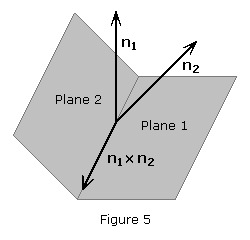
\includegraphics[width=0.6\textwidth]{img/directorrectaimplicitas.jpg}
\caption{Vector director de una recta dada por sus ecuaciones implícitas.}
\label{fig::vectordirectorrectaimplicitas}
\end{figure}

Dada una recta $r$ que pertenece a ambos planos, $\pi_1$ y $\pi_2$, $\vec{v_r}\perp n_{\pi_1} \wedge \vec{v_r}\perp n_{\pi_2}$ (Ver \fref{fig::vectordirectorrectaimplicitas}).
%
Por eso, para buscar un vector perpendiculamr a la vez a 2 vectores dados, el camino más corto es el producto vectorial.

\[\vec{v_r} = n_{\pi_1}\times n_{\pi_2}\]

\begin{problem}

Dada las rectas $r:\left\{\begin{array}{c}2x+y=2\\2y-z=2\end{array}\right.$ y $s:(x,y,z) = (1,1,1) + (-1,2,4)\lambda$.

\solution

Aunque se puede hacer de muchas maneras diferentes, vamos a aplicar el resultado que acabamos de ver.

Los planos que forman la recta $r$ son $\pi_1: 2x+y=2 \text{ con } \vec{n_{\pi_1}} = (2,1,0)$ y $\pi_2: 2y-z=2 \text{ con } \vec{n_{\pi_2}} = (0,2,-1)$ 

Obtenemos $\vec{v_r} = (2,1,0)\times (0,2,-1) = \crossprodandcalc{2}{1}{0}{0}{2}{-1}$

Tenemos $\vec{v_r} \;||\; \vec{v_s}$. Estudiamos $P_s \in r$:

\[
\left\{\begin{array}{c}2·1+1\neq2\\2·1-1\neq2\end{array}\right. \implies P_s\not\in r\implies r\;||\;s \text{ no coincidentes.}
\]
\end{problem}



\obs Fíjate que podríamos haber obtenido $\vec{v_r}$ parametrizando. ¿Cuándo es más corto parametrizar y cuándo utilizar el producto vectorial?

\begin{problem}
Dadas las siguientes rectas, obtén un vector director por el camino más corto

\ppart $r_1:\left\{\begin{array}{c}2x+y=2\\2y-z=2\end{array}\right.$
\ppart $r_2:\left\{\begin{array}{c}2x+5y+z=2\\3x-2y-7z=2\end{array}\right.$
\ppart $r_3:\left\{\begin{array}{c}x+y+z=2\\x-y-z=2\end{array}\right.$

\solution


\end{problem}


\paragraph{Problemas recomendados: T12 - 127,128}

\begin{problem}[Junio 2019]

Dados los puntos $A(1,1,1), B(1,3,-3)$ y $C(-3,-1,1)$, se pide:
\ppart Determinar la ecuación del plano que contiene a los 3 puntos.
\ppart Obtener un punto $D$ (distinto a los anteriores) tal que los vectores $\vec{AB}$, $\vec{AC}$,$\vec{AD}$ sean linealmente dependientes.
\ppart Encontrar un punto $P$ del eje $OX$, de modo que el volumen del tetraedro de vértices $A$,$B$,$C$,$P$ sea igual a 1.

\solution

\spart 

Tomamos $\vec{AB} = (0,2,-4)$, $\vec{AC} = (-4,-2,0)$ como vectores directores del plano y calculamos su ecuación implícita:

\[
\pi: \left|\begin{array}{ccc}
x - 1 & 0 & -4\\
y - 1 & 2 & -2\\
z - 1 & -4& 0
\end{array}\right| = 0 \dimplies 16y-16 + 8z-8-8x+8 = 0\]
\[\dimplies -8x + 16y + 8z -16 = 0 \dimplies -x+2y+z-2=0
\]

\spart Basta con tomar $D\in\pi$. Por ejemplo: $D(0,1,0)\in\pi$.

Comprobamos que $\vec{AB},\vec{AC},\vec{AD}$ son linealmente dependientes calculando el determinante de la matriz que forman.

$\vec{AD} = (1,0,1)$

\[
|\vec{AB}\quad\vec{AC}\quad\vec{AD}| = 
\left|\begin{array}{ccc}
1 & 0 & -4\\
0 & 2 & -2\\
1 & -4& 0
\end{array}\right| = 0
\]

\spart 

(Ojo que aquí no se puede simplificar, aunque antes sí hubiéramos podido)

Buscamos $P(a,0,0)$. El volumen del tetraedro será $\rfrac{1}{6}$ del voluen del paralelepípedo.

\[
\left|\left|\vec{AP}\quad\vec{AB}\quad\vec{AC}\right|\right| = 6 \dimplies
\left|\left|\begin{array}{ccc}
a-1 & 0 & -4\\
-1 & 2 & -2\\
-1 & -4& 0
\end{array}\right|\right| = 2·2·\left|\left|\begin{array}{ccc}
a-1 & 0 & 2\\
-1 & 1 & 1\\
-1 & -2& 0
\end{array}\right|\right| = {6} 
\]
\[
 \left|\left|\begin{array}{ccc}
a-1 & 0 & 2\\
-1 & 1 & 1\\
-1 & -2& 0
\end{array}\right|\right| = \frac{3}{2}  \dimplies |2a+4| = \rfrac{3}{2} \implies\]
\[
\left\{\begin{array}{c}
4+2a_1 = -\rfrac{3}{2} \dimplies a_1 = \frac{-11}{4} \to P_1\left(\rfrac{-11}{4},0,0\right)\\
4+2a_2 = \rfrac{3}{2} \dimplies a_2 = \frac{-5}{4} \to P_2\left(\rfrac{-5}{4},0,0\right)
\end{array}\right.
\]

\end{problem}


\subsection{Proyecciones y simetrías}

\subsubsection{Proyección}

\paragraph{Proyección de punto sobre plano}
\index{Proyección!punto sobre plano}

Para calcular la proyección de un punto $P$ sobre un plano $\pi$ (ver \fref{fig::proy::punto-plano}):
\begin{enumerate}
  \item $r\perp \pi$ con $P\in r$
  \item $P' = r\cap \pi$
\end{enumerate}

\begin{figure}[H]
\centering
\tdplotsetmaincoords{60}{110}

\begin{tikzpicture}[tdplot_main_coords,scale=0.8]
    % draw axes
    \fill[blue!20!white] (-2,-2,0) to (5,-2,0) to (5,5,0) node[anchor=south,color=black]{$\pi$} to (-2,5,0)to cycle;
    \draw[dashed,color=black!45!white] (2,2,-1) -- (2,2,4) node[anchor=west]{$r\perp\pi$};
    \draw[fill] (2,2,3) circle(1pt) node[anchor=west]{$P$};
    \draw[fill,color=red] (2,2,0) circle(1pt) node[anchor=west]{$P'$};
\end{tikzpicture}
\caption{Proyección de punto sobre plano}
\label{fig::proy::punto-plano}
\end{figure}

\paragraph{Proyección de recta sobre plano}
\index{Proyección!recta sobre plano}

Se reduce a proyectar 2 puntos de la recta sobre el plano. Se puede utilizar el punto de intersección de la recta con el plano.

\obs Buenas prácticas: calcular el punto de intersección para saber si la recta pertenece al plano o es paralela. 
\begin{itemize}
  \item Si $r\in\pi$, la proyección de la recta será ella misma.
  \item Si $r\;||\;\pi$, necesitaremos proyectar 2 puntos de la recta.
  \item En los demás casos, se proyecta un punto sobre la recta y la proyección será la que pasa por el punto proyectado y el punto de intersección. Ver \fref{fig::proy::recta-plano}.
\end{itemize}

\begin{figure}[H]
\centering
\tdplotsetmaincoords{60}{110}
\begin{tikzpicture}[tdplot_main_coords,scale=0.8]
    % draw axes
    \fill[blue!20!white] (-2,-2,0) to (6,-2,0) to (6,6,0) node[anchor=south,color=black]{$\pi$} to (-2,6,0)to cycle;
    \draw (0,0,0) -- (2.5,5,5) node[anchor=west]{$r$};
    \draw[dashed] (-1,-2,-2) -- (0,0,0);
    \draw[fill] (0,0,0)circle(2pt) node[anchor=south]{$Q$};
    \draw[fill] (2,4,4)circle(2pt) node[anchor=north west]{$P$};
    \draw[fill] (2,4,0) circle(2pt) node[anchor=north]{$P'$};
    \draw[dashed] (2,4,4) -- (2,4,0);
    \draw[color=red] (-1,-2,0) -- (2.5,5,0) node[anchor=north east]{$r'$};  
\end{tikzpicture}
\caption{Proyección de recta sobre plano}
\label{fig::proy::recta-plano}
\end{figure}


\begin{problem}

Dada la recta $r:\left\{\begin{array}{c}2x+y+z=1\\x+2y+z=2\end{array}\right.$ y el plano $\pi:2x+2y+z=2$, halla la proyección de $r$ sobre $\pi$

\solution

\ul{Cálculo intersección $r\cap\pi$}
\textit{Seguimos el consejo de buenas prácticas.}

\[
\left\{\begin{array}{c}
2x+y+z=1\\
x+2y+z=2\\
2x+2y+z=2
\end{array}\right\} \overset{E_3-E_2}{\dimplies}
\left\{\begin{array}{c}
2x+y+z=1\\
x+2y+z=2\\
x=0
\end{array}\right\} \overset{E_1-E_2}\dimplies 
\left\{\begin{array}{c}
2x+y+z=1\\
x-y=-1\\
x=0
\end{array}\right\}  \dimplies\]\[
\left\{\begin{array}{c}
2x+y+z=1\\
y=1\\
x=0
\end{array}\right\} \to A = \pi\cap r = (0,1,0)\]

Ya tenemos un punto de la recta buscada. Necesitamos hallar la proyección de un $P_r$ sobre el plano.

\ul{Cálculo de proyección de un punto $P_r$}

1) Tomamos $x=1$ y sustituimos en $r$ para hallar $P_r$

\[
\left\{\begin{array}{c}2x+y+z=1\\x+2y+z=2\end{array}\right\}\to
\left\{\begin{array}{c}
y+z=-1\\
2y+z=1
\end{array}\right\}\overset{E_2-E_1}\dimplies
\left\{\begin{array}{c}
y+z=-1\\
y=2
\end{array}\right\}\to (x,y,z) = (1,2,-3)
\]

2) Buscamos $t\perp\pi$ con $P_r\in t$. 

\[
t:\left\{\vec{n_{\pi}},P_r \right\}:\left\{
\begin{array}{c}
x=1+2\lambda
y=2+2\lambda
z=-3+\lambda
\end{array}
\right\}
\]

3) La recta proyección será la formada por $A$ y $B=t\cap\pi$ 

\[
B: 2(1+2\lambda)+2(2+2\lambda)+(-3+\lambda)=2 \dimplies 9\lambda+3=2\dimplies \lambda=\rfrac{-1}{9}
\]

Así, $B\left(1+2\rfrac{-1}{9},2+2\rfrac{-1}{9},-3+\rfrac{-1}{9}\right)$ 

\ul{Conclusión:}
$A (0,1,0)$ y $B\left(\rfrac{7}{9},\rfrac{16}{9},\rfrac{-28}{9}\right)$ forman la recta $r$.


$\vec{AB} = \left(\rfrac{7}{9},\rfrac{7}{9},\rfrac{-28}{9}\right)$. Como $\vec{AB} \;||\; (7,7,-28) \;||\; (1,1,-4)$ tomamos como $\vec{v} = (1,1,-4)$

\[
\text{Solución: }r:\{A,\vec{v}\}:
\left\{\begin{array}{l}
x=\lambda\\
y=1+\lambda\\
z=-4\lambda
\end{array}
\right.
\]
\end{problem}



\paragraph{Proyección de punto sobre recta:}
\index{Proyección!punto sobre recta}

\begin{figure}[H]
\centering
\tdplotsetmaincoords{60}{110}
\begin{tikzpicture}[tdplot_main_coords,scale=0.8]
    % draw axes
    \fill[blue!20!white] (-4,0,-2) to (4,0,-2) to (4,0,4) node[anchor=south,color=black]{$\pi$} to (-4,0,4)to cycle;
    \draw (0,0,0) -- (0,4,0) node[anchor=east]{$r$};
    \draw[dashed] (0,-1.6,0) -- (0,0,0);
    \draw (0,-1.6,0)--(0,-3,0);
    \draw[fill,color=red] (0,0,0)circle(2pt) node[anchor=north]{$P'$};
    \draw[fill] (0,0,3)circle(2pt) node[anchor=west]{$P$};
    \draw[dashed] (0,0,0) -- (0,0,3);
\end{tikzpicture}
\caption{Proyección de punto sobre recta}
\label{fig::proy::punto-recta}
\end{figure}


\begin{problem}
Página 311, ejercicio 11
\solution
\end{problem}

\subsubsection{Simetría de un punto respecto de otro punto}
\index{Simetría!punto respecto de punto}

Todo el cálculo de objetos simétricos respecto de otros se va a basar en este caso, el caso más simple.

\begin{figure}[H]
\centering
\tdplotsetmaincoords{60}{110}
\begin{tikzpicture}[tdplot_main_coords,scale=0.8]
    % draw axes
    %\fill[blue!20!white] (-2,-2,0) to (6,-2,0) to (6,6,0) node[anchor=south,color=black]{$\pi$} to (-2,6,0)to cycle;
    \draw[dashed] (0,3,0) -- (0,0,0);
    \draw[dashed] (0,-3,0) -- (0,3,0);
    \draw[fill,color=red] (0,-3,0)circle(2pt) node[anchor=south]{$P'$};
    \draw[fill] (0,3,0)circle(2pt) node[anchor=south]{$P$};
    \draw[fill] (0,0,0) circle(2pt) node[anchor=south]{$M_{PP'}$};
\end{tikzpicture}
\caption{Simetría de un punto respecto de otro punto}
\label{fig::sim::punto-punto}
\end{figure}


\begin{problem}

Dado el punto $A(2,3,4)$ halla su simétrico respecto de $B(1,1,1)$.

\solution

Buscamos $A'$ que cumpla que $B$ es el punto medio entre $A$ y $A'(x,y,z)$.

Sabemos que el punto medio entre $P$ y $Q$ tiene coordenadas:$M_{PQ}\left(\frac{p_1+q_1}{2},\frac{p_2+q_2}{2},\frac{p_3+q_3}{2}\right)$

Resolvemos:

\[
\left(\frac{2+x}{2},\frac{3+y}{2},\frac{4+z}{2}\right) = (1,1,1) \dimplies ... \dimplies (x,y,z) = (0,-1,-2)
\]

\end{problem}


\subsubsection{Simetría de un punto respecto de una recta}
\index{Simetría!punto respecto de recta}

Plano perpendicular a la recta que contenga al punto, intersección con la recta (ver \fref{fig::sim::punto-recta}).

\begin{figure}[H]
\centering
\tdplotsetmaincoords{60}{110}
\begin{tikzpicture}[tdplot_main_coords,scale=0.8]
    % draw axes
    \fill[blue!20!white] (-4,0,-4) to (4,0,-4) to (4,0,4) node[anchor=south,color=black]{$\pi$} to (-4,0,4)to cycle;
    \draw (0,0,0) -- (0,4,0) node[anchor=east]{$r$};
    \draw[dashed] (0,-1.6,0) -- (0,0,0);
    \draw (0,-1.6,0)--(0,-3,0);
    
    \draw[fill] (0,0,2)circle(2pt) node[anchor=west]{$P$};
    \draw[fill] (0,0,0)circle(2pt) node[anchor=north]{$M_{PP'}$};
    \draw[fill,color=red] (0,0,-2)circle(2pt) node[anchor=west]{$P'$};
    \draw[dashed] (0,0,-2) -- (0,0,2);
\end{tikzpicture}
\caption{Simetría de punto respecto de recta}
\label{fig::sim::punto-recta}
\end{figure}


\subsubsection{Simetría de un punto respecto de un plano}
\index{Simetría!punto respecto de un plano}

Recta perpendicular al plano, que pasa por el punto (ver \fref{fig::sim::punto-plano}).

\begin{figure}[H]
\centering
\tdplotsetmaincoords{60}{110}
\begin{tikzpicture}[tdplot_main_coords,scale=0.8]
    % draw axes
    \fill[blue!20!white] (-2,-2,0) to (5,-2,0) to (5,5,0) node[anchor=south,color=black]{$\pi$} to (-2,5,0)to cycle;
    \draw(2,2,1) -- (2,2,3);
    \draw(2,2,0) -- (2,2,1) node[anchor=west]{$r\perp\pi$};
    \draw[dashed](2,2,-2) -- (2,2,0);
    \draw(2,2,-3) -- (2,2,-2);
    \draw[fill] (2,2,3)circle(1pt) node[anchor=east]{$P$};
    \draw[fill] (2,2,0) circle(1pt) node[anchor=north east]{$M_{PP'}$};
    \draw[fill,color=red] (2,2,-3) circle(1pt) node[anchor=east]{$P'$};
\end{tikzpicture}
\caption{Simétrico de punto respecto de un plano}
\label{fig::sim::punto-plano}
\end{figure}



\subsubsection{Simetría de una recta respecto de un plano}
\index{Simetría!recta respecto de plano}

\begin{figure}[H]
\centering
\tdplotsetmaincoords{60}{110}

\begin{tikzpicture}[tdplot_main_coords,scale=0.8]
    % draw axes
    \fill[blue!20!white] (-2,-2,0) to (6,-2,0) to (6,6,0) node[anchor=south,color=black]{$\pi$} to (-2,6,0)to cycle;
    \draw (0,0,0) -- (2.5,5,5) node[anchor=east]{$r$};
    \draw[dashed] (-1,-2,-2) -- (0,0,0);
    \draw[fill] (0,0,0)circle(2pt) node[anchor=south]{$Q$};
    \draw[fill] (2,4,4)circle(2pt) node[anchor=north west]{$P$};
    \draw[fill] (2,4,0) circle(2pt) node[anchor=north]{$M_{PP'}$};
    \draw[fill] (2,4,-4) circle(2pt) node[anchor=north]{$P'$};
    \draw[dashed] (2,4,4) -- (2,4,-4);
    \draw[color=red] (-1,-2,2) -- (0,0,0);  
    \draw[color=red,dashed] (0,0,0) -- (1.4,2.8,-2.8) node[anchor=north east]{$r'$};  
    \draw[color=red] (1.4,2.8,-2.8) -- (2,4,-4) ;  
\end{tikzpicture}
\caption{Simetría de una recta respecto de un plano}
\label{fig::sim::recta-plano}
\end{figure}


\begin{problem}

Halla la recta simétrica de $r$ respecto del plano $\pi: 2x+2z=0$.

\[r: \begin{cases}x=1+\lambda\\y=1-\lambda\\z=\lambda\end{cases}\]

\solution


\end{problem}


\newpage
\subsection{Ángulos}
\subsubsection{Ángulo formado por dos rectas}
\index{Ángulo!formado por dos rectas}

Llamamos ángulo formado por 2 rectas al menor de los 2 ángulos que forman (en la \fref{fig::ang-recta-recta}, llamaríamos $\widehat{r,s} = \alpha$). Según su posición relativa se distinguen:

\begin{itemize}
  \item \textbf{Secantes:} el ángulo de las rectas será el ángulo de los vectores directores.
  \item \textbf{Paralelas/coincidentes:} ángulo 0.
  \item \textbf{Rectas que se cruzan:} el ángulo que forman es el que forman 2 paralelas a ellas que sean secantes. 
\end{itemize}

Se calcula el ángulo desde la definición de producto escalar.

\[
\cos(\alpha) = \cos(\hat{r,s}) = \left| \cos\left(\hat{\vec{v_r},\vec{v_s}}\right)\right| = \frac{|\vec{v_r}·\vec{v_s}|}{|\vec{v_r}|·|\vec{v_s}|} \implies 0\leq \alpha \leq \rfrac{\pi}{2}
\]


\begin{figure}[H]
\centering
\tdplotsetmaincoords{60}{110}
\begin{tikzpicture}[scale=0.8]
    % draw axes
\coordinate (a) at (0,0);
\coordinate (b) at (3,2);
\coordinate (c) at (0,3);

\draw pic[draw,fill=green!30,angle radius=1cm,"$\beta$" shift={(15mm,1mm)}] {angle=c--a--b};
\draw pic[draw,fill=blue!30,angle radius=0.5cm,"$\alpha$" shift={(3mm,4mm)}] {angle=b--a--c};

\draw  (-3,-2) -- (a) -- node[above] {$r$} (b);
\draw  (0,-3) -- (a) -- node[above right] {$s$} (c);
\end{tikzpicture}
\caption{Ángulo formado por 2 rectas}
\label{fig::ang-recta-recta}
\end{figure}


\subsubsection{Ángulo formado por dos planos}
\index{Ángulo!formado por dos planos}

Llamamos ángulo formado por 2 planos al menor de los 2 ángulos diedros que forman 2 planos secantes (ver \fref{fig::ang-plano-plano}).

\obs Si los planos son paralelos, no forman ningún ángulo.

\[
\cos(\alpha) = \cos\left(\widehat{\pi_1,\pi_2}\right) = \left|\cos\left(\widehat{\vec{n_1},\vec{n_2}}\right)\right| = \frac{|\vec{n_1}·\vec{n_2}|}{|\vec{n_1}|·|\vec{n_2}|} \implies 0\leq \alpha \leq \rfrac{\pi}{2}
\]

\begin{figure}[H]
\centering
%\tdplotsetmaincoords{60}{110}
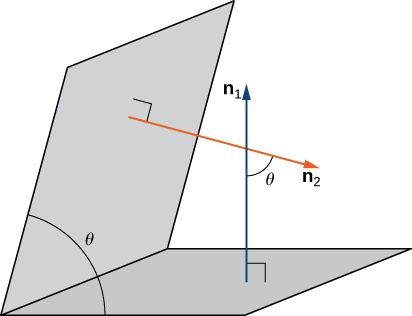
\includegraphics[width=0.6\textwidth]{img/angle-between-planes.jpeg}
%\input{tikz/ang-plano-plano.tex}
\caption{Ángulo formado por 2 planos}
\label{fig::ang-plano-plano}
\end{figure}


\subsubsection{Ángulo formado por recta y plano}
\index{Ángulo!formado por recta y un plano}

\begin{itemize}
  \item Sería posible calcular el ángulo que forma la recta con su proyección. Ver \fref{fig::ang-recta-plano}.
  \item Otra posibilidad, utilizar el vector normal del plano: $\widehat{r,\pi} = 90º-\widehat{r,\vec{n_{\pi}}}$
\end{itemize}


\begin{figure}[H]
\centering
\tdplotsetmaincoords{60}{110}
\begin{tikzpicture}[tdplot_main_coords,scale=0.8]
    % draw axes
    \coordinate (P) at (2,4,4);
    \coordinate (O) at (0,0,0);
    \coordinate (Q) at (2,4,0);

    % draw axes
    \fill[blue!20!white] (-2,-2,0) to (6,-2,0) to (6,6,0) node[anchor=south,color=black]{$\pi$} to (-2,6,0)to cycle;
    \draw (0,0,0) -- (2.5,5,5) node[anchor=east]{$r$};
    \draw[dashed] (-1,-2,-2) -- (0,0,0);
    \draw[fill] (0,0,0)circle(2pt) node[anchor=south]{$Q$};
    \draw[fill] (2,4,4)circle(2pt) node[anchor=north west]{$P$};
    \draw[fill] (2,4,0) circle(2pt) node[anchor=north]{$P_{\pi}$};
    
    \draw[dashed] (2,4,4) -- (2,4,0);


    \draw[color=red,dashed] (-1,-2,0) -- (0,0,0);  
    \draw[color=red,dashed] (0,0,0) -- (1.4,2.8,0) node[anchor=north east]{$r_{\pi}$};  
    \draw[color=red,dashed] (1.4,2.8,0) -- (2.5,5,0); 


    \pic [color=green!30!black,fill=green!30!black,draw, ->, "$\alpha$", angle eccentricity=1.5] {angle = Q--O--P};
    %\fill[color=green!30!black] (0,0,0) -- (-0.5,0,0) -- (-0.635,0.35,0) -- cycle;
\end{tikzpicture}
\caption{Ángulo formado por una recta y un plano}
\label{fig::ang-recta-plano}
\end{figure}

\begin{problem}

Calcula el ángulo formado por la recta $r$ y el plano $\pi$.

\[
r : \begin{cases} 2x-3y+z=0\\x-z=0\end{cases}\;\;\;\pi: x+y-2z=3
\]
\solution

Obtenemos las ecuaciones paramétricas de la recta, calculando las soluciones del sistema compatible indeterminado:

\[
r : \begin{cases} 2x-3y+z=0\\x-z=0\end{cases} \overset{x=\lambda}{\to}
\begin{cases} 2\lambda-3y+\lambda = 0 \to y=\lambda \\x=z=\lambda\end{cases} \dimplies \begin{cases}x=\lambda\\y=\lambda\\z=\lambda\end{cases}
\]

\ul{Método 1: Angulo entre vectores}

\[
\widehat{\pi,\vec{v_r}} = 90 - \widehat{\vec{n_{\pi}},\vec{v_r}}
\]

\[
\cos\left(\widehat{\vec{n_{\pi}},\vec{v_r}}\right) = \frac{|\vec{n_{\pi}}·\vec{v_r}|}{|\vec{n_{\pi}}|·|\vec{v_r}|} = \frac{(1,1,1)·(1,1,-2)}{\sqrt{1^2+1^2+1^2}·\sqrt{1^2+1^2+(-2)^2}} = 0 
\]

\[
\cos\left(\widehat{\vec{n_{\pi}},\vec{v_r}}\right) = 0\implies \widehat{\vec{n_{\pi}},\vec{v_r}} = 90 \implies \widehat{\pi,\vec{v_r}} = 0 \implies \pi\;||\; r
\]


\ul{Método 2: Ángulo con la proyección} (no merece la pena)

Para calcular la proyección de una recta sobre un plano:
\begin{enumerate}
  \item Comprobamos $r\in \pi: \lambda+\lambda-2\lambda = 3 \nexists\lambda\in\real\implies r\;||\;\pi$ con $r\cap\pi=\emptyset$ 
  
  \item Varias opciones:
  \subitem a) Necesitamos proyectar 2 puntos de la recta sobre el plano. Tomamos los puntos $A(0,0,0)\in r$ y $B(1,1,1)\in r$.

  \textbf{$A_{\pi}$:} Calculamos $t\perp\pi (\implies \vec{v_t}\;||\;\vec{n_{\pi}})$ con $A\in t\to t\begin{cases}x=\lambda\\y=\lambda\\z=-2\lambda\end{cases}$

  Calculamos $t\cap\pi: \lambda+\lambda+4\lambda=3\dimplies \lambda=\rfrac{1}{2} \implies t\cap\pi =A_{\pi}=\left(\rfrac{1}{2},\rfrac{1}{2},-1\right)$

  \textbf{$B_{\pi}$:} Calculamos $t'\perp\pi (\implies \vec{v_t'}\;||\;\vec{n_{\pi}})$ con $B\in t'\to t'\begin{cases}x=1+\mu\\y=1+\mu\\z=1-2\mu\end{cases}$

  Calculamos $t'\cap\pi: (1+\mu)+(1+\mu)-2(1-2\mu)=3\dimplies \mu=\rfrac{1}{2} \implies t\cap\pi =B_{\pi}=\left(\rfrac{3}{2},\rfrac{3}{2},0\right)$

  Calculamos $r_{\pi}:\{A,\vec{AB}\} \dimplies r:\begin{cases}x=\rfrac{1}{2}+\lambda\\y=\rfrac{1}{2}+\lambda\\z=\rfrac{1}{2}+\lambda\end{cases}$

\obs ¿Es casualidad que $\vec{v_r} = \vec{v_{r_{\pi}}}$? No, una recta paralela a un plano y su proyección sobre ese plano son rectas paralelas, por lo que tienen vectores directores proporcionales.
\end{enumerate}

\end{problem}



\subsubsection{Perpendicular común}

Ver \fref{fig::Perpendicularcomun}. Buscamos la recta $t$, perpendicular a la vez a $s$ y a $r$, que las corte. 

Para ello:
\begin{itemize}
  \item $\vec{v_t} = \vec{v_r}\times\vec{v_s}$
  \item Dado que encontrar los puntos de intersección es muy complejo, podemos recurrir a construir 2 planos.
  \begin{itemize}
    \item $\pi_1: \{\vec{v_t},\vec{v_r},P_r\}$
    \item $\pi_2: \{\vec{v_t},\vec{v_s},P_s\}$
  \end{itemize}
  Así, $t:\{\pi_1,\pi_2\}$
\end{itemize}

\begin{problem}
Video de unicoos.
\solution

\end{problem}


\begin{figure}[H]
\centering
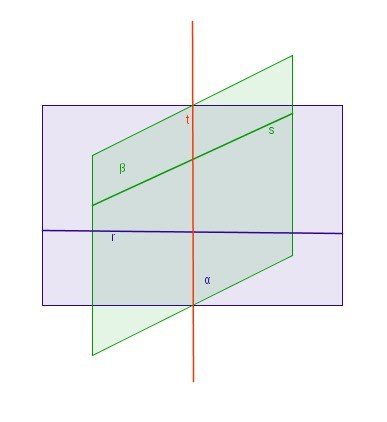
\includegraphics[scale=0.7]{img/PerpendicularComun.jpg}
\caption{Perpendicular común}
\label{fig::Perpendicularcomun}
\end{figure}

\subsubsection{Recta que corta a 2 rectas y pasa por un punto.}

%Vídeo de unicoos para ver en casa (si funciona el anterior).


\subsection{Distancias}
\subsubsection{Entre 2 puntos}
Módulo del vector.

\subsubsection{Entre punto y plano}

La distancia entre el punto y su proyección sobre el plano. Ver \fref{fig::dist-punto-plano}.
\index{Distancia!punto-plano}


\begin{itemize}
  \item $d(P,\pi) = |PP_{\pi}|$, siendo $P_{\pi}$ la proyección del punto sobre el plano.
  \item Se puede utilizar otro camino más corto para calcular esta distancia. Ver \fref{fig::dist-punto-plano}.

  \subitem Consideramos $Q\in\pi$.
  \subitem $|\vec{n_{\pi}}·\vec{QP}| = |\vec{n_{\pi}}|·|\vec{QP}|·\cos(\alpha)$, siendo $\alpha$ el ángulo que forman estos vectores.
  \subitem Aplicando la definición de coseno: $\cos(\alpha) = \rfrac{d(P,\pi)}{|\vec{QP}|}$.
  \subitem Sustituyendo y despejando: $|\vec{n_{\pi}}·\vec{QP}| = |\vec{n_{\pi}}|·d(P,\pi) \to d(P,\pi) = \frac{|\vec{n_{\pi}}·\vec{QP}|}{|\vec{n_{\pi}}|}$
  \subitem $|\vec{n_{\pi}}·\vec{QP}| = |A(p_1-q_1) + B(p_2-q_2) + C(p_3-q_3)| = Ap_1+Bp_2+Cp_3+D$
  \subitem \textbf{Conclusión:}\index{Distancia! punto-plano}

  \[
    d(P,\pi) = \frac{|Aq_1+Bq_2+Cq_3+D|}{|(A,B,C)|}
  \]
\end{itemize}

\begin{figure}[H]
\centering
\tdplotsetmaincoords{60}{110}
\begin{tikzpicture}[tdplot_main_coords,scale=0.8]
    % draw axes
    \fill[blue!20!white] (-2,-2,0) to (6,-2,0) to (6,6,0) node[anchor=south,color=black]{$\pi$} to (-2,6,0)to cycle;
    \draw[->] (0,0,0) -- (2,4,4) node[anchor=south east]{$\overset{\to}{PQ}$};
    \draw[fill] (0,0,0)circle(2pt) node[anchor=south]{$Q$};
    \draw[fill] (2,4,4)circle(2pt) node[anchor=north west]{$P$};
    \draw[fill] (2,4,0) circle(2pt) node[anchor=north]{$P_{\pi}$};
    \draw[->] (0,0,0) -- (2,4,0);
    \draw (1,2,0) node[anchor=north east]{$\overset{\to}{QP_{\pi}}$};
    \draw[dashed] (2,4,4) -- (2,4,0);
    \draw[->,color=red!50!black] (2,4,0) -- (2,4,2) node[anchor=west]{$n_{\pi}$};
\end{tikzpicture}
\caption{Distancia de un punto a un plano}
\label{fig::dist-punto-plano}
\end{figure}


\[d(P,\pi) = \frac{|Ap_1+Bp_2+Cp_3+D|}{|(A,B,C)|}\]

\subsubsection{Entre 2 planos o entre una recta y un plano}
\index{Distancia!plano-plano}
\index{Distancia!recta-plano}

\begin{itemize}
  \item Se comprueba si son paralelos (porque sino, distancia 0).
  \item Si no lo son, calculamos la distancia entre un punto que pertenezca al plano o a la recta y al otro plano.
\end{itemize}


\begin{figure}[H]
\centering
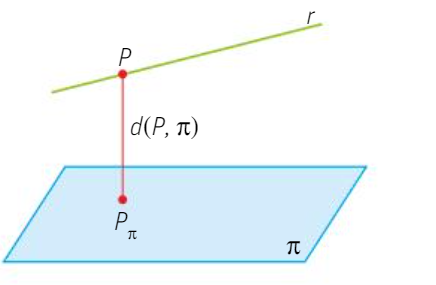
\includegraphics[scale=0.6]{img/dist-recta-plano.png}
\caption{Distancia de una recta a un plano paralelo}
\label{fig::dist-recta-plano}
\end{figure}


\subsubsection{Entre punto y recta}
\index{Distancia!punto-recta}

\begin{itemize}
  \item $d(P,r) = |PP_{r}|$, siendo $P_r$ la proyección de $P$ sobre $r$.
  \item Otra manera de calcular sería considerar un punto $Q\in r$. Ver \fref{fig::dist-punto-recta}.
  \subitem Considerando $\vec{QP}$ y $\vec{v_r}$ (ambos fáciles de calcular), $d(P,r)$ se podría calcular utilizando la definición de seno. Así,
  
  \[\sen\left(\widehat{\vec{v_r},\vec{QP}}\right) = \displaystyle\frac{|d(P,r)|}{|\vec{QP}|}\]

  \subitem Utilizando $|\vec{QP}\times\vec{v_r}| = |\vec{QP}|·|\vec{v_r}|\sen(\alpha)$, despejamos:
  \[
    |\vec{QP}\times\vec{v_r}| = |\vec{QP}|·|\vec{v_r}|·\frac{|d(P,r)|}{|\vec{QP}|} \dimplies d(P,r) = \frac{|\vec{QP}\times\vec{v_r}|}{|\vec{v_r}|}
  \]
\end{itemize}

\begin{figure}[H]
\centering
\tdplotsetmaincoords{60}{110}
\begin{tikzpicture}[scale=1.2]
    % draw axes
    \draw (-3,0) to (3,0) node[anchor=north]{$r$};
    \draw[fill] (-1,0)circle(1pt) node[anchor=south]{$Q$};

    \draw[fill] (1,0)circle(1pt) node[anchor=north west]{$P_{r}$};
    \draw[fill] (1,2)circle(1pt) node[anchor=west]{$P$};
    \draw[->] (-1,0) -- (0,0) node[anchor=north]{$\overset{\to}{v_r}$};
    \draw[->] (1,0) -- (1,2);
    \draw(1,1) node[anchor=west]{$d(P,r)$};
    \draw[->] (-1,0) -- (1,2);
    \draw(0,1.5) node{$\overset{\to}{PQ}$};
\end{tikzpicture}
\caption{Distancia de un punto a una recta}
\label{fig::dist-punto-recta}
\end{figure}



\subsubsection{Entre 2 rectas}
\index{Distancia!recta-recta}
\begin{itemize}
  \item Si $r\cap s \neq \emptyset \implies d(r,s) = 0$
  \item Comprobamos si $r\;||\;s$. 
  \subitem Si $r\;||\;s \implies d(r,s) = d(P_r,s) = d(P_s,r)$
  \subitem Si $r\;\not||\; s \implies d(r,s) = d(r,\pi)$, con $\pi:\{v_r,v_s,P_s\}$
\end{itemize}

\begin{figure}[H]
\centering
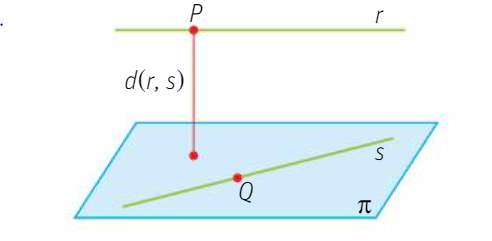
\includegraphics[scale=0.6]{img/dist-recta-recta-cruzan.png}
\caption{Distancia entre 2 rectas que se cruzan}
\label{fig::dist-rectas-cruzan}
\end{figure}


\subsection{Lugares geométricos}


\subsubsection{Plano mediador}

Es el \lgdlp dos puntos $A$ y $B$. Utilizando la definición, consideramos un punto genérico $P(x,y,z)$ al que obligamos a cumplir que 
\[\pi: d(P,A) = d(P,B) \dimplies\]
\[\pi: +\sqrt{(x-a_1)^2+(y-a_2)^2+(z-a_3)^2} = +\sqrt{(x-a_1)^2+(y-a_2)^2+(z-a_3)^2} \dimplies\]
\[\pi: (x-a_1)^2+(y-a_2)^2+(z-a_3)^2 = (x-a_1)^2+(y-a_2)^2+(z-a_3)^2\dimplies ...\]

\paragraph{Otra opción: } Podemos considerar $\pi:\{\vec{AB} = n_{\pi}, M_{AB}\}$ 

\begin{figure}[H]
\centering
\tdplotsetmaincoords{60}{110}
\begin{tikzpicture}[tdplot_main_coords,scale=0.8]
    % draw axes
    \fill[blue!20!white] (-2,-2,0) to (5,-2,0) to (5,5,0) to (-2,5,0) node[anchor=south,color=black]{$\pi_{AB}$} to cycle;
    \draw(2,2,1) -- (2,2,3);
    \draw(2,2,0) -- (2,2,1);
    \draw[dashed](2,2,-2) -- (2,2,0);
    \draw(2,2,-3) -- (2,2,-2);
    \draw[fill] (2,2,3)circle(1pt) node[anchor=east]{$A$};
    \draw[fill] (2,2,0) circle(1pt) node[anchor=north east]{$M_{AB}$};
    \draw[fill] (2,2,-3) circle(1pt) node[anchor=east]{$B$};
    \draw (3,4.5,0) circle(1pt) node[anchor=west]{$P(x,y,z)$};
    \draw[dashed,color=gray] (2,2,3) to (3,4.5,0);
    \draw[dashed,color=gray] (2,2,-3) to (3,4.5,0);
\end{tikzpicture}
\caption{Plano mediador de un segmento.}
\label{fig::plano-mediador}
\end{figure}



\subsubsection{Planos bisectores}

Es el \lgdlp 2 planos $\pi$ y $\tau$. 
%
Utilizando la definición, consideramos un punto genérico $P(x,y,z)$ al que obligamos a cumplir que 

\[d(P,\pi) = d(P,\tau) \dimplies \frac{|A_{\pi}x + B_{\pi}y+C_{\pi}z+D|}{\sqrt{A_{\pi}^2+B_{\pi}^2+C_{\pi}^2}} =  \frac{|A_{\tau}x + B_{\tau}y+C_{\tau}z+D|}{\sqrt{A_{\tau}^2+B_{\tau}^2+C_{\tau}^2}}\]

Dado que $|A| = |B| \dimplies \left\{\begin{array}{c}A=B\\A=-B\end{array}\right\}$, tenemos:

\[
\begin{cases}
\displaystyle\frac{A_{\pi}x + B_{\pi}y+C_{\pi}z+D}{\sqrt{A_{\pi}^2+B_{\pi}^2+C_{\pi}^2}} =  +\frac{A_{\tau}x + B_{\tau}y+C_{\tau}z+D}{\sqrt{A_{\tau}^2+B_{\tau}^2+C_{\tau}^2}}
\\
\displaystyle\frac{A_{\pi}x + B_{\pi}y+C_{\pi}z+D}{\sqrt{A_{\pi}^2+B_{\pi}^2+C_{\pi}^2}} = - \frac{A_{\tau}x + B_{\tau}y+C_{\tau}z+D}{\sqrt{A_{\tau}^2+B_{\tau}^2+C_{\tau}^2}}
\end{cases}
\]

Hay 2 soluciones.

\begin{figure}[H]
\centering
\tdplotsetmaincoords{60}{110}
\begin{tikzpicture}[tdplot_main_coords,scale=0.8]
    % draw axes
    \fill[red!90!white, opacity=0.7] (0,0,0) to (1,0,0) to (1,2,0) to (0,2,0)to cycle;
    \fill[yellow!100!white, opacity=0.9] (1,0,-2) to (1,0,2) to (1,2,2) to (1,2,-2) to cycle;
    \fill[red!90!white, opacity=0.7] (1,0,0) to (2,0,0) to (2,2,0) to (1,2,0)to cycle;
    \draw (1,-0.5,0) to (1,2.5,0) ;
    \draw (1,3,0.5) node{$\to$};
\end{tikzpicture}
\begin{tikzpicture}[tdplot_main_coords,scale=0.8]
    % draw axes
    \fill[blue!20!white, opacity=0.7] (1,0,0) to (0,0,-2) to (0,2,-2) to (1,2,0)to cycle;
    \fill[yellow!100!white, opacity=0.9] (1,0,-2) to (1,0,2) to (1,2,2) to (1,2,-2) to cycle;
    \fill[red!90!white, opacity=0.7] (-0.3,0,0) to (1,0,0) to (1,2,0) to (-0.3,2,0)to cycle;
    %\fill[purple!80!white, opacity=0.7] (1,2,0) to (0,0,1) to (-1,-1,-2) to (1,0,0)to cycle;
    \fill[blue!50!white, opacity=0.7] (1,2,0) to (2,2,-1) to (2,0,-1) to (1,0,0)to cycle;
    \fill[blue!50!white, opacity=0.7] (1,2,0) to (0,2,1) to (0,0,1) to (1,0,0)to cycle;
    \fill[red!90!white, opacity=0.7] (1,0,0) to (2.25,0,0) to (2.25,2,0) to (1,2,0)to cycle;
    \draw (1,-0.5,0) to (1,2.5,0) ;
    \fill[yellow!100!white, opacity=0.9] (1,0,-0) to (1,0,2) to (1,2,2) to (1,2,-0) to cycle;
    \fill[blue!20!white, opacity=0.7] (1,0,0) to (2,0,2) to (2,2,2) to (1,2,0)to cycle;
\end{tikzpicture}
\caption{En azul, olos planos bisectores de un diedro.}
\label{fig::planos-bisectores}
\end{figure}

\begin{problem}
Calcula la ecuación de los planos que dividen a los diedros determinados por los planos $\pi:2x+y-2z=1$ y $\pi': 2x+2y+z=5$ en dos partes iguales.
\solution
Sea $P(x,y,z)$

\[d(P,\pi) = d(P,\pi') \dimplies \frac{|2x+y-2z-1|}{\sqrt{4+1+4}} = \frac{|2x+2y+z-5|}{\sqrt{4+4+1}} \dimplies |2x+y-2z-1| = |2x+2y+z-5|\]

\[
\begin{cases}
2x+y-2z-1 = 2x+2y+z-5\\
2x+y-2z-1 =-\left(2x+2y+z-5\right)
\end{cases}\implies 
\begin{cases}
\tau_1: y+3z-4 = 0\\
\tau_2: 4x+3y-z-6=0
\end{cases}
\]


\obs ¿Qué ángulo forman los 2 planos bisectores? La intuición dice que deberían ser perpendiculares, igual que, en 2 dimensiones, las bisectrices de 2 rectas son perpendiculares. 
%
Vamos a demostrarlo.

\[
\tau_1 \perp\tau_2 \dimplies \vec{n_{\tau_1}} \perp \vec{n_{\tau_2}} \dimplies \vec{n_{\tau_1}}·\vec{n_{\tau_2}} = 0
\]

Comprobamos $\vec{n_{\tau_1}}·\vec{n_{\tau_2}} = (0,1,3)·(4,3,-1) = 3-3=0\implies \tau_1 \perp\tau_2 $

¿Qué ocurre si los planos iniciales, $\pi,\pi'$, son paralelos? En ese caso solo existe un único plano bisector. Vamos a verlo en otro problema diferente.
\end{problem}

\begin{problem}

Determina el lugar geométrico de los puntos del espacio que equidistan de los planos $\pi: x+y+z+4=0$ y $\pi':2x+2x+2z+4=0$.

\solution

Sea $P(x,y,z)$

\[
  d(P,\pi) = d(P,\pi') \dimplies \frac{|x+y+z+4|}{\sqrt{1+1+1}} = \frac{|2x+2y+2z+4|}{\sqrt{4+4+4}} \dimplies 
\]
\[
  \frac{|x+y+z+4|}{\sqrt{3}} = \frac{|2x+2y+2z+4|}{2\sqrt{3}} \dimplies 2·|x+y+z+4| = |2x+2y+2z+4|\dimplies 
\]
\[
\begin{cases}
  2x+2y+2z+8=2x+2y+2z+4 \to \nexists \tau_1\\
  2x+2y+2z+8=-2x-2y-2z-4 \to 4x+4y+4z+12 = 0 \dimplies \tau_2: x+y+z+3=0
\end{cases}
\]

Solo se ha obtenido una solución, debido a que $\pi\;||\;\pi'$.
\end{problem}


\begin{table}[h]
\centering
\begin{tabular}{|c|c|c|}
\hline
\textbf{Definición} & \textbf{Solución} & \textbf{Este curso}\\\hline
2 puntos & Plano mediador & Sí\\\hline
2 plano & Plano bisector & Sí\\\hline
2 rectas paralelas & Plano ¿mediador? & Sí\\\hline
2 rectas que se cruzan & Ver \fref{fig::lgdlp-rectas-cruzan} & No \\\hline
1 puntos & Superficie esférica & Sí, pero no\\\hline
1 recta & Superficie cilíndrica & No\\\hline
1 plano & No tiene solución & \\\hline
\end{tabular}
\caption{\lgdlp...}
\label{tbl::lugaresgeometricos}
\end{table}

\begin{figure}[H]
\centering
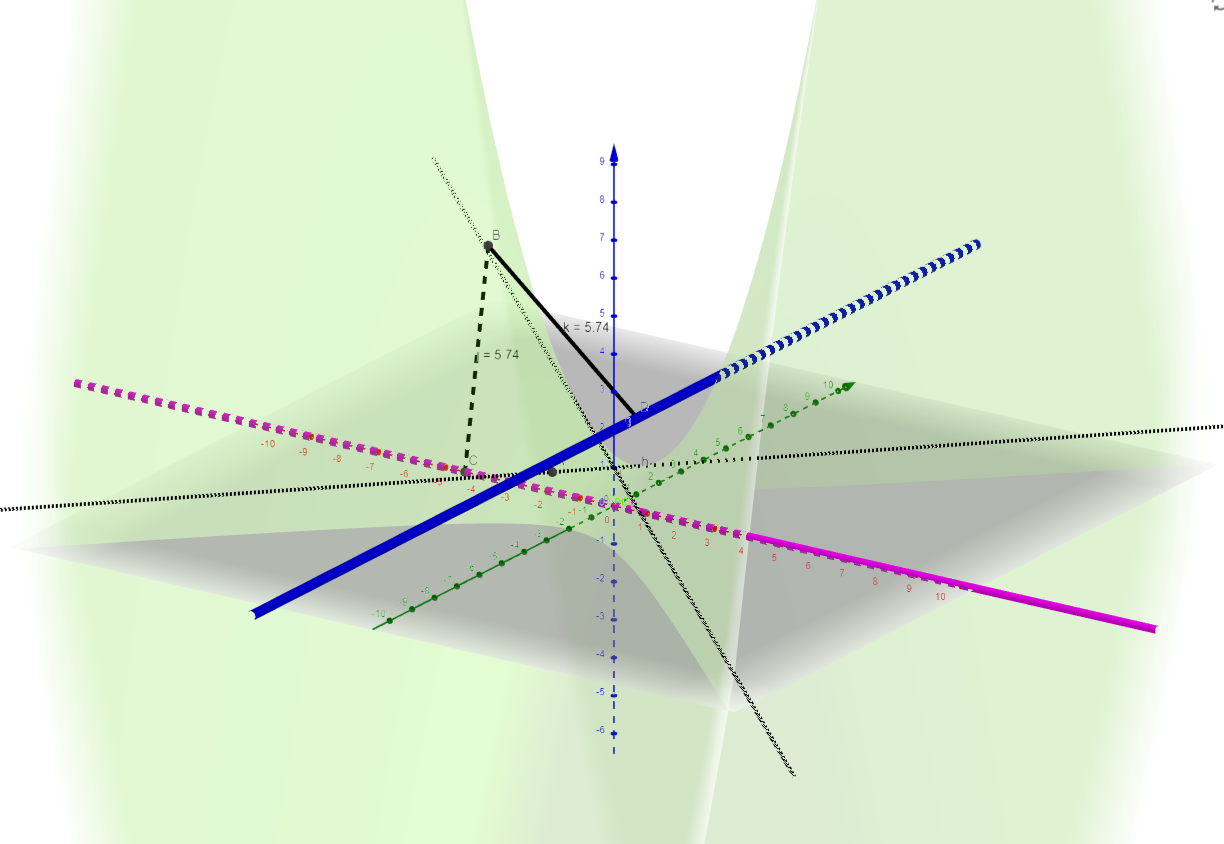
\includegraphics[scale=0.6]{img/lgdlprectascruzan.png}
\caption{Representación geométrica del lugar geométrico de los puntos del epacio que equidistan. Para ver en 3 dimensiones, consultar: https://www.geogebra.org/m/rabpxx8t}
\label{fig::lgdlp-rectas-cruzan}
\end{figure}


\subsection{Áreas y volúmenes}
\begin{itemize}
  \item Área del paralelogramo: $\left|\vec{a}\times\vec{b}\right|$
  \item Área del triángulo: $\rfrac{1}{2}·\left|\vec{a}\times\vec{b}\right|$
  \item Volumen del paralelepípedo: $\left|[\vec{a},\vec{b},\vec{c}]\right|$
  \item Volumen del tetraedro: $\rfrac{1}{6}[\vec{a},\vec{b},\vec{c}]$
\end{itemize}


\begin{problem}
Halla la ecuación de la recta que pasa por el punto $P(2,0,-1)$ y corta a las rectas $r$ y $s$, siendo:

\[r:\frac{x-2}{2} = \frac{y-2}{-1} = \frac{z+1}{1}\]
\[s:\begin{cases}x+y+4=0\\y-3z+3=0\end{cases}\]
\solution
Vídeo de unicoos.

\ul{Plan b:} Método alternativo: mates con Andrés.
\end{problem}
